\documentclass{article}

\usepackage[left=1.5in, right=1.5in, top=1in, bottom=1in]{geometry}
\usepackage{graphicx}
\usepackage{amsmath}
\usepackage{amssymb}
\usepackage{hyperref}

\usepackage{graphicx}
\graphicspath{ {./img/} }

\usepackage[backend=biber]{biblatex}
\bibliography{sources.bib}

\title{Mathematical Models of Delta-Notch Signalling}  
\author{Riley Wheadon, Edwin Huras, Ziyi Zhuang}

\begin{document}

\maketitle

\begin{flushleft}

\section{Abstract}

The Delta-Notch signalling pathway plays a critical role in determining the cell fate of initially homogeneous cells in diverse biological systems. Early deterministic models of Delta-Notch interactions, such as that by Collier et al. (1996), achieved cell differentiation in linear and 2D cell arrays. In this paper, we develop a simple – yet more biologically realistic – ODE model of Delta-Notch signalling and compare the deterministic behaviour with the Collier et al. model. We derive a probabilistic framework via Kolmogorov forward equations, demonstrating that, in expectation, it converges to our ODE model under appropriate limiting conditions. By comparing deterministic ODEs, stochastic ODEs, and Gillespie simulations, we show that natural perturbations in receptor-ligand binding dynamics are sufficient to produce differentiation, even from identical initial conditions. Numerical experiments across parameter regimes highlight the robustness of this behaviour and bifurcation analysis further reveals the parameter-dependent bistability.

\section{Introduction}

\medskip

Binding of the Delta ligand from cell $B$ to the Notch receptor on cell $A$ results in the \emph{cleavage} (removal) of both the ligand and receptor \cite{collier_pattern_1996}. This interaction triggers the release of NICD (Notch Intracellular Domain) in cell $A$, which \emph{promotes} Notch and \emph{inhibits} Delta.

\begin{itemize}
  \item The Serrate (Jagged) ligand can also bind to Notch. Unlike Delta, NICD promotes Jagged, which creates a double-positive feedback loop.
  \item Interaction between Delta ligands and Notch receptors from the same cell (cis-interaction) removes both molecules and does not trigger the release of NICD.
\end{itemize}

\subsection{Model}

Collier et al. make the following five modelling assumptions:
\begin{enumerate}
  \item Cells interact through Delta-Notch signalling if and only if they are adjacent.
  \item Production of Notch is an increasing (hill) function of Delta in neighbouring cells.
  \item Production of Delta is a decreasing (hill) function of Notch in the same cell.
  \item Production of Notch and Delta is balanced by decay proportional to concentration.
  \item Low levels of Notch cause the primary fate, high levels cause the secondary fate.
\end{enumerate}

Then they define the following variables:

\begin{itemize}
  \item $\tau$: time
  \item $N_{P}$: notch activity (concentration) in cell $P$
  \item $D_{P}$: delta activity (concentration) in cell $P$
  \item $\overline{D}_{P}$: average delta activity in neighbours of $P$
  \item $N_{0}$: typical notch activity (across all cells)
  \item $D_{0}$: typical delta activity (across all cells)
  \item $\mu$: The decay rate for notch (assumed constant)
  \item $\rho$: The decay rate for delta (assumed constant)
\end{itemize}

Then, define the following system of differential equations, where $F:[0, \infty) \rightarrow [0, \infty)$ is a continuous increasing function and $G: [0, \infty)\rightarrow [0, \infty)$ is a continuous decreasing function.

$$
\begin{aligned}
  \frac{d(N_{P} / N_{0})}{d\tau} = F(\overline{D}_{P} / D_{0}) - \mu N_{P} / N_{0} \\[5pt]
  \frac{d(D_{P} / D_{0})}{d\tau} = G(N_{P} / N_{0}) - \rho D_{P} / D_{0}
\end{aligned}
$$

This equation is inherently nondimensional, since $N_{P} / N_{0}$ and $D_{P} / D_{0}$ have no units.

\subsection{Issues}

The Collier et al. model makes numerous simplifications that violate our current understanding of the delta-notch signalling network. These simplifications make it difficult to derive a probabilistic model from the Collier et al. model, since the biological implications of such a model would be contradictory. Some of the issues include:

\begin{itemize}
  \item Production of activated Notch (NICD) is exclusively a function of the Delta concentration in neighbouring cells, with no regard for the concentration of extracellular Notch receptors.
  \item Furthermore, the concentration of extracellular Notch isn't accounted for at all, which means there is no way to create a meaningful reaction term that captures the dynamics of the system.
  \item There are smaller issues, like the absence of cis-inhibition and the Serrate (Jagged) protein, but these aren't necessary to capture the fundamental behaviour of the system.
\end{itemize}

\subsection{Qualitative Results}

In the two-cell periodic boundary condition case, Collier et al. show that there always exists a homogeneous steady state, although this state is unstable if the feedback in the Delta-Notch signalling network is sufficiently strong. If the line of cells is given Dirichlet boundary conditions, the inhomogeneity arises on the outside edges before gradually spreading inwards to the center of the domain. On the two-dimensional hexagonal lattice, the system exhibits different ratios of primary to secondary fated cells depending on the parameters. In particular, Collier et al. observed ratios of $1/2$, $1/3$, $1/4$, $1/5$, and $1/6$.

\section{Methods}

\subsection{Parameters and Assumptions}

Assume \emph{a priori} (i.e. from previous research) the following, where $I$ is NICD:

\begin{itemize}
  \item Basal extracellular Notch ($N$) production has the form $H^{+}(I) = n_{m}I^2/(n_{0}^2 + I^2)$. 
  \item Basal extracellular Delta ($D$) production has the form $H^{-}(I) = d_{m}d_{0}^2/(d_{0}^2 + I^2)$.
  \item Extracellular Notch and Delta have the same decay rate, $\gamma$.
\end{itemize}

Then, define the following parameters:

\begin{itemize}
  \item $N_{0}$ and $D_{0}$ are the maximum rates of Notch/Delta production.
  \item $k_{T}$ is the binding rate between extracellular Notch and Delta.
  \item $N_{ext}$ and $D_{ext}$ refer to the average Notch/Delta levels in neighbouring cells.
  \item $\gamma_{I}$ is the decay rate of NICD.
\end{itemize}

\newpage

Furthermore, we will assume that there is no cis-interaction and no Serrate ligand. This gives us the following set of chemical reactions that can occur in a single time step:

\begin{enumerate}
  \item A Notch receptor (from cell $A$) binds to a Delta ligand (from cell $B$), triggering the release of NICD in cell $A$. This can be written as $N_{A} + D_{B} \rightarrow I_{A}$. The probability of this event is $k_{T}N_{A}D_{B}$.
  \item A Notch receptor in cell $A$ decays ($N_{A} \rightarrow \emptyset$) with probability $\gamma N_{A}$.
  \item A Delta ligand in cell $A$ decays ($D_{A} \rightarrow \emptyset$) with probability $\gamma D_{A}$.
  \item A NICD molecule in cell $A$ decays ($I_{A} \rightarrow \emptyset$) with probability $\gamma_{I}I_{A}$.
  \item A Notch receptor in cell $A$ is produced ($\emptyset \rightarrow N_{A}$) with probability $H^{+}(I)$.
  \item A Delta ligand in cell $A$ is produced ($\emptyset \rightarrow D_{A}$) with probability $H^{-}(I)$.
\end{enumerate}

\subsection{Kolmogorov Forward Equations}
\subsubsection{Derivation of Kolmogorov Forward Equation}

Let us define:\\
$P(n,d,i,t)$ = probability of having $n$ Notch receptors, $d$ Delta ligands, and $i$ NICD molecules at time $t$.\\

The Kolmogorov forward equation describes how $P(n,d,i,t)$ changes over a small time step $\Delta t$:

\begin{align*}
P(n,d,i,t+\Delta t) &= P(n,d,i,t) \\
&+ P(n-1,d,i,t) \cdot H^+(i) \Delta t \quad \text{(Notch production)} \\
&+ P(n,d-1,i,t) \cdot H^-(i) \Delta t \quad \text{(Delta production)} \\
&+ P(n+1,d,i,t) \cdot \gamma(n+1)\Delta t \quad \text{(Notch decay)} \\
&+ P(n,d+1,i,t) \cdot \gamma(d+1)\Delta t \quad \text{(Delta decay)} \\
&+ P(n,d,i+1,t) \cdot \gamma_I(i+1)\Delta t \quad \text{(NICD decay)} \\
&+ P(n+1,d,i-1,t) \cdot k_T(n+1)D_{ext}\Delta t \quad \text{(Trans-activation)} \\
&- P(n,d,i,t) \cdot [H^+(i) + H^-(i) + \gamma n + \gamma d + \gamma_I i + k_T n D_{ext}]\Delta t
\end{align*}

Rearranging to find the time derivative:

\begin{align*}
\frac{P(n,d,i,t+\Delta t) - P(n,d,i,t)}{\Delta t} &= P(n-1,d,i,t) \cdot H^+(i) \\
&+ P(n,d-1,i,t) \cdot H^-(i) \\
&+ P(n+1,d,i,t) \cdot \gamma(n+1) \\
&+ P(n,d+1,i,t) \cdot \gamma(d+1) \\
&+ P(n,d,i+1,t) \cdot \gamma_I(i+1) \\
&+ P(n+1,d,i-1,t) \cdot k_T(n+1)D_{ext} \\
&- P(n,d,i,t) \cdot [H^+(i) + H^-(i) + \gamma n + \gamma d + \gamma_I i + k_T n D_{ext}]
\end{align*}

Taking the limit as $\Delta t \rightarrow 0$:

\begin{align*}
\frac{\partial P(n,d,i,t)}{\partial t} &= P(n-1,d,i,t) \cdot H^+(i) \\
&+ P(n,d-1,i,t) \cdot H^-(i) \\
&+ P(n+1,d,i,t) \cdot \gamma(n+1) \\
&+ P(n,d+1,i,t) \cdot \gamma(d+1) \\
&+ P(n,d,i+1,t) \cdot \gamma_I(i+1) \\
&+ P(n+1,d,i-1,t) \cdot k_T(n+1)D_{ext} \\
&- P(n,d,i,t) \cdot [H^+(i) + H^-(i) + \gamma n + \gamma d + \gamma_I i + k_T n D_{ext}]
\end{align*}

\subsubsection{Matrix Formulation}
The Kolmogorov forward equation can be expressed in matrix form as:
\[
\frac{d\vec{P}(t)}{dt} = \mathbf{A} \vec{P}(t)
\]

where $\vec{P}(t)$ is a column vector containing the probabilities for all possible states, and $\mathbf{A}$ is the transition rate matrix. \\

To construct the matrix $\mathbf{A}$, we first establish a one-to-one mapping between the three-dimensional state space $(n,d,i)$ and a one-dimensional index $k$. For a system with maximum values $n_{max}$, $d_{max}$, and $i_{max}$, we define:
\[
k(n,d,i) = n \cdot (d_{max}+1) \cdot (i_{max}+1) + d \cdot (i_{max}+1) + i
\]
for $0 \leq n \leq n_{max}, \; 0 \leq d \leq d_{max}, \; 0 \leq i \leq i_{max}$.

The inverse mapping gives:
\begin{align*}
n(k) &= \left\lfloor \frac{k}{(d_{max}+1) \cdot (i_{max}+1)} \right\rfloor \\
d(k) &= \left\lfloor \frac{k \bmod ((d_{max}+1) \cdot (i_{max}+1))}{i_{max}+1} \right\rfloor \\
i(k) &= k \bmod (i_{max}+1)
\end{align*}

With this mapping, we can now define the elements of matrix $\mathbf{A}$. Let $k$ and $k'$ be the indices corresponding to states $(n,d,i)$ and $(n',d',i')$ respectively:

\begin{align*}
A_{k',k} = 
\begin{cases}
H^+(i) & \text{if } (n',d',i') = (n+1,d,i) \quad \text{(Notch production)} \\
H^-(i) & \text{if } (n',d',i') = (n,d+1,i) \quad \text{(Delta production)} \\
\gamma(n) & \text{if } (n',d',i') = (n-1,d,i) \quad \text{(Notch decay)} \\
\gamma(d) & \text{if } (n',d',i') = (n,d-1,i) \quad \text{(Delta decay)} \\
\gamma_I(i) & \text{if } (n',d',i') = (n,d,i-1) \quad \text{(NICD decay)} \\
k_T(n)D_{ext} & \text{if } (n',d',i') = (n-1,d,i+1) \quad \text{(Trans-activation)} \\
-\sum_{k'' \neq k} A_{k'',k} & \text{if } k' = k \quad \text{(Diagonal terms)}
\end{cases}
\end{align*}

Note that $A_{k',k}$ represents the transition rate from state $k$ to state $k'$. The diagonal elements $A_{k,k}$ are the negative sum of all outgoing rates from state $k$:

\[
A_{k,k} = -[H^+(i) + H^-(i) + \gamma n + \gamma d + \gamma_I i + k_T n D_{ext} + k_T d N_{ext}]
\]

where $(n,d,i)$ is the state corresponding to index $k$.\\

The resulting matrix $\mathbf{A}$ is a sparse matrix with the following properties:
\begin{itemize}
    \item Dimension: $(n_{max}+1) \cdot (d_{max}+1) \cdot (i_{max}+1) \times (n_{max}+1) \cdot (d_{max}+1) \cdot (i_{max}+1)$
    \item Number of non-zero elements: $\approx 7 \cdot (n_{max}+1) \cdot (d_{max}+1) \cdot (i_{max}+1)$
\end{itemize}

To illustrate, let's consider a minimal system with $n_{max} = d_{max} = i_{max} = 1$. This gives us 8 possible states:
$(0,0,0)$, $(0,0,1)$, $(0,1,0)$, $(0,1,1)$, $(1,0,0)$, $(1,0,1)$, $(1,1,0)$, $(1,1,1)$

The corresponding transition matrix $\mathbf{A}$ would be:

\begin{align*}
\mathbf{A} = 
\begin{pmatrix}
-\alpha_{000} & \gamma_I & \gamma & 0 & \gamma & 0 & 0 & 0 \\
H^+(0) & -\alpha_{001} & 0 & \gamma & 0 & \gamma & 0 & 0 \\
H^-(0) & 0 & -\alpha_{010} & \gamma_I & 0 & 0 & \gamma & 0 \\
0 & H^-(0) & H^+(0) & -\alpha_{011} & 0 & 0 & 0 & \gamma \\
H^+(0) & 0 & 0 & 0 & -\alpha_{100} & \gamma_I & \gamma & 0 \\
0 & H^+(0) & 0 & 0 & H^+(1) & -\alpha_{101} & 0 & \gamma \\
0 & 0 & H^+(0) & 0 & H^-(1) & 0 & -\alpha_{110} & \gamma_I \\
0 & 0 & 0 & H^+(0) & 0 & H^-(1) & H^+(1) & -\alpha_{111}
\end{pmatrix}
\end{align*}

where:
\[
\alpha_{ndi} = H^+(i) + H^-(i) + \gamma n + \gamma d + \gamma_I i + k_T n D_{ext} + k_T d N_{ext}
\]

Additionally, we need to add the terms for trans-activation, which would connect states like $(1,0,0)$ to $(0,0,1)$ with rate $k_T \cdot 1 \cdot D_{ext}$.\\

For a fully labelled matrix with all transitions explicitly shown, the matrix for $n_{max} = d_{max} = i_{max} = 1$ would be:

\[
\mathbf{A} = 
\begin{bmatrix}
A_{11} & A_{12} & A_{13} & A_{14} & A_{15} & A_{16} & A_{17} & A_{18} \\
B_{11} & B_{12} & B_{13} & B_{14} & B_{15} & B_{16} & B_{17} & B_{18} \\
C_{11} & C_{12} & C_{13} & C_{14} & C_{15} & C_{16} & C_{17} & C_{18} \\
D_{11} & D_{12} & D_{13} & D_{14} & D_{15} & D_{16} & D_{17} & D_{18} \\
E_{11} & E_{12} & E_{13} & E_{14} & E_{15} & E_{16} & E_{17} & E_{18} \\
F_{11} & F_{12} & F_{13} & F_{14} & F_{15} & F_{16} & F_{17} & F_{18} \\
G_{11} & G_{12} & G_{13} & G_{14} & G_{15} & G_{16} & G_{17} & G_{18} \\
H_{11} & H_{12} & H_{13} & H_{14} & H_{15} & H_{16} & H_{17} & H_{18}
\end{bmatrix}
\]

where  

\begin{tiny}
\begin{align*}
A_{11} &= -(H^+(0) + H^-(0)),  & A_{12} &= \gamma_I,  \\
A_{13} &= \gamma,  & A_{14} &= 0,  \\
A_{15} &= \gamma,  & A_{16} &= 0,  \\
A_{17} &= 0,  & A_{18} &= 0,  \\[5pt]
B_{11} &= H^+(0),  & B_{12} &= -(H^+(1) + H^-(1) + \gamma_I),  \\
B_{13} &= 0,  & B_{14} &= \gamma,  \\
B_{15} &= k_T D_{ext},  & B_{16} &= \gamma,  \\
B_{17} &= 0,  & B_{18} &= 0,  \\[5pt]
C_{11} &= H^-(0),  & C_{12} &= 0,  \\
C_{13} &= -(H^+(0) + H^-(0) + \gamma + k_T N_{ext}),  & C_{14} &= \gamma_I,  \\
C_{15} &= 0,  & C_{16} &= 0,  \\
C_{17} &= \gamma,  & C_{18} &= 0,  \\[5pt]
D_{11} &= 0,  & D_{12} &= H^-(1),  \\
D_{13} &= H^+(0),  & D_{14} &= -(H^+(1) + H^-(1) + \gamma + \gamma_I + k_T N_{ext}),  \\
D_{15} &= 0,  & D_{16} &= k_T D_{ext},  \\
D_{17} &= 0,  & D_{18} &= \gamma,  \\[5pt]
E_{11} &= H^+(0),  & E_{12} &= 0,  \\
E_{13} &= 0,  & E_{14} &= 0,  \\
E_{15} &= -(H^+(0) + H^-(0) + \gamma + k_T D_{ext}),  & E_{16} &= \gamma_I,  \\
E_{17} &= \gamma,  & E_{18} &= 0,  \\[5pt]
F_{11} &= 0,  & F_{12} &= H^+(1),  \\
F_{13} &= 0,  & F_{14} &= 0,  \\
F_{15} &= H^+(0),  & F_{16} &= -(H^+(1) + H^-(1) + \gamma + \gamma_I + k_T D_{ext}),  \\
F_{17} &= 0,  & F_{18} &= \gamma,  \\[5pt]
G_{11} &= 0,  & G_{12} &= 0,  \\
G_{13} &= H^+(0),  & G_{14} &= 0,  \\
G_{15} &= H^-(0),  & G_{16} &= 0,  \\
G_{17} &= -(H^+(0) + H^-(0) + \gamma + \gamma + k_T D_{ext} + k_T N_{ext}),  & G_{18} &= \gamma_I,  \\[5pt]
H_{11} &= 0,  & H_{12} &= 0,  \\
H_{13} &= 0,  & H_{14} &= H^+(1),  \\
H_{15} &= 0,  & H_{16} &= H^-(1),  \\
H_{17} &= H^+(0),  & H_{18} &= -(H^+(1) + H^-(1) + \gamma + \gamma + \gamma_I + k_T D_{ext} + k_T N_{ext}).
\end{align*}
\end{tiny}

Each row and column corresponds to a state in the order:
$(0,0,0)$, $(0,0,1)$, $(0,1,0)$, $(0,1,1)$, $(1,0,0)$, $(1,0,1)$, $(1,1,0)$, $(1,1,1)$

The matrix element $A_{j,i}$ represents the transition rate from state $i$ to state $j$. The diagonal elements $A_{i,i}$ contain the negative sum of all outgoing rates from state $i$.

\subsection{Deterministic ODE Model}

We implemented the following deterministic ODE model adapted from Boareto et al. (2015): 

$$
\begin{aligned}
  \frac{dN}{dt} &= \frac{n_{m}I^2}{n_{0}^2 + I^2} - k_{T}ND_{ext} - \gamma N \\[5pt]
  \frac{dD}{dt} &= \frac{d_{m}d_{0}^2}{d_{0}^2 + I^2} - k_{T}DN_{ext} - \gamma D \\[5pt]
  \frac{dI}{dt} &= k_{T}ND_{ext} - \gamma_{I}I
\end{aligned}
$$

where $N$ is the number of intracellular Notch molecules, $D$ is the number of intracellular Delta molecules, and $I$ is the number of NICD molecules (see $3.1$ reference). This model is a simplification of the model found in Boareto et al. That model included an additonal equation for the Jagged molecule and kept track of cis-inhibition: where a Notch and Delta bind together inside the same cell, resulting in the degradation of both cells without contributing to the amount of NICD. So as to more directly compare our results with those of Collier et al., we ignore Jagged interactions and cis-inhibition. Including an NICD variable was necessary, however, as this additional interaction allowed for the assignment of probabilities to each reaction event and thus for the derivation of the Kolmogorov Equations and Gillespie algorithm.

\subsection{Stochastic ODE Model}

To capture the inherent randomness in cellular processes while maintaining computational efficiency, we implement a stochastic differential equation (SDE) model based on the chemical Langevin equation formalism. This approach represents an intermediate level of detail between the deterministic ODE model and the fully discrete Gillespie algorithm.

Starting from the deterministic ODEs described in Section 3.3, we incorporate stochastic fluctuations by adding noise terms proportional to the square root of the reaction propensities:
$$
\begin{aligned}
  dN &= \left( \frac{n_{m}I^2}{n_{0}^2 + I^2} - k_{T}ND_{ext} - \gamma N \right) dt + \sigma \cdot N \cdot dW_{N} \\ \\[5pt]
  dD &= \left( \frac{d_{m}d_{0}^2}{d_{0}^2 + I^2} - k_{T}DN_{ext} - \gamma D \right)  dt + \sigma \cdot D \cdot dW_{D}  \\[5pt]
  dI &= \left( k_{T}ND_{ext} - \gamma_{I}I \right) dt + \sigma \cdot I \cdot dW_{I}
\end{aligned}
$$
where $dW_N$, $dW_D$, and $dW_I$ are independent Wiener processes representing white noise. The structure of the noise terms follows from the assumption that noise in each reaction channel is proportional to the current concentration of those molecules. \par

For numerical implementation, we employ the Euler-Maruyama scheme with time step $dt$. The deterministic step is first calculated, and then the Wiener increments are sampled from a normal distribution with mean 0 and standard deviation $\sqrt{dt}$. Each increment is scaled by the its respective variable and added to the results of the deterministic step.

\subsection{Gillespie Algorithm}

We will make the assumption that reaction times follow a Poisson point process. Let $E$ be the set of all possible reaction events (i.e. reactions 1-6 above for all cells). Furthermore, let $|E| = N$ be the number of possible reactions. For each event, let $X_{i} \sim \text{Exp}(\lambda_{i})$ denote the time until the next event of type $i$, where $1 \leq i \leq N$. Then, the waiting time $T$ in between \emph{any} two events is:

$$
T = \text{min} \{ X_{1}, \dots, X_{N} \} \sim \text{Exp}\left( \sum_{i = 1}^{N} \lambda_{i} \right) 
$$

This results follows from the definition of an exponential distribution and the memoryless property. Then, we can use Gillespie's algorithm to simulate the system as follows:

\medskip

\textbf{Step 1}: Sample a value $t_{i}$ from $T$ using inverse transform sampling. 

\medskip

\textbf{Step 2}: Increment the current time $t$ by $t_{i}$.

\medskip

\textbf{Step 3}: Determine which event took place. To do this, recall that:

$$P(X_{k} = \text{min} \{  X_{1}, \dots, X_{N} \}) = \frac{\lambda_{k}}{\lambda_{1} + \dots + \lambda_{N}}$$

Use this fact to partition the interval $[0, 1]$. Then sample $y_{i}$ from a $\text{Unif}(0, 1)$ distribution, identify its partition, and find the corresponding event.

\medskip

\textbf{Step 4}: Update the state based on the event determined in the previous step.

\medskip

\textbf{Remark}: The expected time for event $i$ to occur is given by $\mathbb{E}[X_{i}] = 1/\lambda_{i}$. Therefore, the rate at which event $i$ occurs is $\lambda_{i}$, which is equal to the rate at which the event occurs in the original ODE. This means that the trajectories generated from the Gillespie's algorithm implementation of the model can be compared directly to the trajectories generated from the ODE itself, without any need for scaling.

\subsection{Theoretical Justification}

In this section, we need to show that in expectation, the model above converges to the following system of ODEs (adapted from Boareto et al., 2015):

$$
\begin{aligned}
  \frac{dN}{dt} &= \frac{n_{m}I^2}{n_{0}^2 + I^2} - k_{T}ND_{ext} - \gamma N \\[5pt]
  \frac{dD}{dt} &= \frac{d_{m}d_{0}^2}{d_{0}^2 + I^2} - k_{T}DN_{ext} - \gamma D \\[5pt]
  \frac{dI}{dt} &= k_{T}ND_{ext} - \gamma_{I}I
\end{aligned}
$$

\subsubsection{Setup and Notation}

Let us define:
\begin{itemize}
  \item $\langle N \rangle = \sum_{n,d,i} n \cdot P(n,d,i,t)$ = expected number of Notch receptors
  \item $\langle D \rangle = \sum_{n,d,i} d \cdot P(n,d,i,t)$ = expected number of Delta ligands
  \item $\langle I \rangle = \sum_{n,d,i} i \cdot P(n,d,i,t)$ = expected number of NICD molecules
\end{itemize}
\subsubsection{Deriving ODEs for Expected Values}

\textbf{Now we derive the ODE for the expected value of Notch:}

\begin{align*}
\frac{d\langle N \rangle}{dt} &= \frac{d}{dt}\sum_{n,d,i} n \cdot P(n,d,i,t) \\
&= \sum_{n,d,i} n \cdot \frac{\partial P(n,d,i,t)}{\partial t}
\end{align*}

Substituting the Kolmogorov forward equation:

\begin{align*}
\frac{d\langle N \rangle}{dt} &= \sum_{n,d,i} n \cdot \Big[ P(n-1,d,i,t) \cdot H^+(i) \\
&+ P(n,d-1,i,t) \cdot H^-(i) \\
&+ P(n+1,d,i,t) \cdot \gamma(n+1) \\
&+ P(n,d+1,i,t) \cdot \gamma(d+1) \\
&+ P(n,d,i+1,t) \cdot \gamma_I(i+1) \\
&+ P(n+1,d,i-1,t) \cdot k_T(n+1)D_{ext} \\
&- P(n,d,i,t) \cdot [H^+(i) + H^-(i) + \gamma n + \gamma d + \gamma_I i + k_T n D_{ext}] \Big]
\end{align*}

Now we use index shifting to simplify.\\~\\

\textbf{(A) Notch Production} \\
Let's substitute $n' = n-1$ (so $n = n'+1$):
\begin{align*}
\sum_{n,d,i} n \cdot P(n-1,d,i,t) \cdot H^+(i) &= \sum_{n',d,i} (n'+1) \cdot P(n',d,i,t) \cdot H^+(i) \\
&= \sum_{n',d,i} n' \cdot P(n',d,i,t) \cdot H^+(i) + \sum_{n',d,i} P(n',d,i,t) \cdot H^+(i) \\
&= \sum_{n,d,i} n \cdot P(n,d,i,t) \cdot H^+(i) + \sum_{n,d,i} P(n,d,i,t) \cdot H^+(i) \\
\end{align*}

The first term is $\langle N \cdot H^+(I) \rangle$. If we assume that $H^+(I)$ is approximately $H^+(\langle I \rangle)$, then this term becomes $\langle N \rangle \cdot H^+(\langle I \rangle)$. The second term is $\langle H^+(I) \rangle \approx H^+(\langle I \rangle)$. 

So the contribution of this term is:
\[
\sum_{n,d,i} n \cdot P(n-1,d,i,t) \cdot H^+(i) \approx \langle N \rangle \cdot H^+(\langle I \rangle) + H^+(\langle I \rangle)
\]

Since we are indexing from 0, and $n-1$ could be negative, the sum should start from $n=1$:

\begin{small}
\begin{align*}
\sum_{n \geq 1,d,i} n \cdot P(n-1,d,i,t) \cdot H^+(i) &= \sum_{n' \geq 0,d,i} (n'+1) \cdot P(n',d,i,t) \cdot H^+(i) \\
&= \sum_{n' \geq 0,d,i} n' \cdot P(n',d,i,t) \cdot H^+(i) + \sum_{n' \geq 0,d,i} P(n',d,i,t) \cdot H^+(i) \\
&= \langle N \rangle \cdot H^+(\langle I \rangle) + H^+(\langle I \rangle) \\
&= H^+(\langle I \rangle) \cdot (1 + \langle N \rangle)
\end{align*}
\end{small}

\textbf{(B) Delta Production}\\
This term does not affect $N$, so the prefactor $n$ remains with the original probability:
\begin{align*}
\sum_{n,d,i} n \cdot P(n,d-1,i,t) \cdot H^-(i) &= \sum_{n,d',i} n \cdot P(n,d',i,t) \cdot H^-(i) \\
&= \langle N \cdot H^-(I) \rangle \\
&\approx \langle N \rangle \cdot H^-(\langle I \rangle)
\end{align*}

\textbf{(C) Notch Decay}
\begin{align*}
\sum_{n,d,i} n \cdot P(n+1,d,i,t) \cdot \gamma(n+1) &= \sum_{n',d,i} (n'-1) \cdot P(n',d,i,t) \cdot \gamma n' \\
&= \gamma \sum_{n',d,i} (n'-1)n' \cdot P(n',d,i,t) \\
&= \gamma \sum_{n',d,i} n'^2 \cdot P(n',d,i,t) - \gamma \sum_{n',d,i} n' \cdot P(n',d,i,t) \\
&= \gamma(\langle N^2 \rangle - \langle N \rangle)
\end{align*}

If we assume that the variance of $N$ is small compared to its mean (which is reasonable for high molecule counts), then $\langle N^2 \rangle \approx \langle N \rangle^2$. So:
\begin{align*}
\gamma(\langle N^2 \rangle - \langle N \rangle) &\approx \gamma(\langle N \rangle^2 - \langle N \rangle) \\
&= \gamma \langle N \rangle (\langle N \rangle - 1)
\end{align*}

\textbf{(D) Delta Decay}
\begin{align*}
\sum_{n,d,i} n \cdot P(n,d+1,i,t) \cdot \gamma(d+1) &= \gamma \sum_{n,d',i} n \cdot P(n,d',i,t) \cdot d' \\
&= \gamma \langle N \cdot D \rangle \\
&\approx \gamma \langle N \rangle \langle D \rangle
\end{align*}

\textbf{(E) NICD Decay}
\begin{align*}
\sum_{n,d,i} n \cdot P(n,d,i+1,t) \cdot \gamma_I(i+1) &= \gamma_I \sum_{n,d,i'} n \cdot P(n,d,i',t) \cdot i' \\
&= \gamma_I \langle N \cdot I \rangle \\
&\approx \gamma_I \langle N \rangle \langle I \rangle
\end{align*}

\textbf{(F) Trans-activation}
\begin{align*}
\sum_{n,d,i} n \cdot P(n+1,d,i-1,t) \cdot k_T(n+1)D_{ext} &= k_T D_{ext} \sum_{n',d,i'} (n'-1) \cdot P(n',d,i',t) \cdot n' \\
&= k_T D_{ext} \sum_{n',d,i'} (n'^2 - n') \cdot P(n',d,i',t) \\
&= k_T D_{ext} (\langle N^2 \rangle - \langle N \rangle) \\
&\approx k_T D_{ext} \langle N \rangle (\langle N \rangle - 1)
\end{align*}

\textbf{(G) Negative Terms}
\begin{align*}
&-\sum_{n,d,i} n \cdot P(n,d,i,t) \cdot [H^+(i) + H^-(i) + \gamma n + \gamma d + \gamma_I i + k_T n D_{ext}] \\
&= -\langle N \cdot H^+(I) \rangle - \langle N \cdot H^-(I) \rangle - \gamma \langle N^2 \rangle - \gamma \langle N \cdot D \rangle - \gamma_I \langle N \cdot I \rangle - k_T D_{ext} \langle N^2 \rangle \\
&\approx -\langle N \rangle \cdot H^+(\langle I \rangle) - \langle N \rangle \cdot H^-(\langle I \rangle) - \gamma \langle N \rangle^2 - \gamma \langle N \rangle \langle D \rangle - \gamma_I \langle N \rangle
\langle I \rangle - k_T D_{ext} \langle N \rangle^2
\end{align*} \\~\\

\textbf{(H) Final Synthesis of $\langle N \rangle$}\\

Combining all these terms:

\begin{align*}
\frac{d\langle N \rangle}{dt} &= H^+(\langle I \rangle) \cdot (1 + \langle N \rangle) + \langle N \rangle \cdot H^-(\langle I \rangle) + \gamma \langle N \rangle (\langle N \rangle - 1) + \gamma \langle N \rangle \langle D \rangle \\
&+ \gamma_I \langle N \rangle \langle I \rangle + k_T D_{ext} \langle N \rangle (\langle N \rangle - 1) \\
&- \langle N \rangle \cdot H^+(\langle I \rangle) - \langle N \rangle \cdot H^-(\langle I \rangle) - \gamma \langle N \rangle^2 - \gamma \langle N \rangle \langle D \rangle - \gamma_I \langle N \rangle \langle I \rangle - k_T D_{ext} \langle N \rangle^2 \\
\end{align*}

After cancellations:

\begin{align*}
\frac{d\langle N \rangle}{dt} &= H^+(\langle I \rangle) + \langle N \rangle \cdot H^+(\langle I \rangle) + \gamma \langle N \rangle (\langle N \rangle - 1) + k_T D_{ext} \langle N \rangle (\langle N \rangle - 1) \\
&- \langle N \rangle \cdot H^+(\langle I \rangle) - \gamma \langle N \rangle^2 - k_T D_{ext} \langle N \rangle^2 \\
&= H^+(\langle I \rangle) + \gamma \langle N \rangle (\langle N \rangle - 1) - \gamma \langle N \rangle^2 + k_T D_{ext} \langle N \rangle (\langle N \rangle - 1) - k_T D_{ext} \langle N \rangle^2 \\
&= H^+(\langle I \rangle) + \gamma \langle N \rangle (\langle N \rangle - 1 - \langle N \rangle) + k_T D_{ext} \langle N \rangle (\langle N \rangle - 1 - \langle N \rangle) \\
&= H^+(\langle I \rangle) - \gamma \langle N \rangle - k_T D_{ext} \langle N \rangle \\
\end{align*}

Therefore, the ODE for $\langle N \rangle$ is:

\[
\frac{d\langle N \rangle}{dt} = H^+(\langle I \rangle) - \gamma \langle N \rangle - k_T D_{ext} \langle N \rangle
\]

Substituting the definition of $H^+(\langle I \rangle)$:

\[
\frac{d\langle N \rangle}{dt} = \frac{n_m \langle I \rangle^2}{n_0^2 + \langle I \rangle^2} - \gamma \langle N \rangle - k_T D_{ext} \langle N \rangle
\]

Which can be written as:

\[
\frac{dN}{dt} = \frac{n_m I^2}{n_0^2 + I^2} - \gamma N - k_T D_{ext} N
\]

where we use $N$, $D$, and $I$ as shorthand for the expected values $\langle N \rangle$, $\langle D \rangle$, and $\langle I \rangle$.\\~\\

\textbf{Similarly, we can derive the ODE for the expected value of Delta:}

\begin{align*}
\frac{d\langle D \rangle}{dt} &= \frac{d}{dt}\sum_{n,d,i} d \cdot P(n,d,i,t) \\
&= \sum_{n,d,i} d \cdot \frac{\partial P(n,d,i,t)}{\partial t}
\end{align*}

We will analyse each term of the Kolmogorov equation, multiplied by $d$, as follows.

\[
\sum_{n,d,i} d \cdot P(n-1,d,i,t) \cdot H^+(i) = \langle D \cdot H^+(I) \rangle \approx \langle D \rangle \cdot H^+(\langle I \rangle)
\]

\[
\sum_{n,d,i} d \cdot P(n,d-1,i,t) \cdot H^-(i) = \langle D \cdot H^-(I) \rangle + \langle H^-(I) \rangle 
\approx \langle D \rangle \cdot H^-(\langle I \rangle) + H^-(\langle I \rangle)
\]

\[
\sum_{n,d,i} d \cdot P(n+1,d,i,t) \cdot \gamma(n+1) \approx \gamma \langle D \rangle \langle N \rangle
\]

\[
\sum_{n,d,i} d \cdot P(n,d+1,i,t) \cdot \gamma(d+1) \approx \gamma \langle D \rangle (\langle D \rangle - 1)
\]

\[
\sum_{n,d,i} d \cdot P(n,d,i+1,t) \cdot \gamma_I(i+1) \approx \gamma_I \langle D \rangle \langle I \rangle
\]

\[
\sum_{n,d,i} d \cdot P(n+1,d,i-1,t) \cdot k_T(n+1)D_{ext} \approx k_T D_{ext} \langle D \rangle \langle N \rangle
\]

Now we consider this term which appears in the ODEs but was not explicitly stated in our Kolmogorov equation setup. This is a special case where we need to account for Delta from our cell binding to Notch in neighbouring cells:

\begin{align*}
-\sum_{n,d,i} d \cdot P(n,d,i,t) \cdot k_T d N_{ext} &= -k_T N_{ext} \sum_{n,d,i} d^2 \cdot P(n,d,i,t) \\
&= -k_T N_{ext} \langle D^2 \rangle \\
&\approx -k_T N_{ext} \langle D \rangle^2
\end{align*}

Now we consider negative terms from original equation.
\begin{align*}
&-\sum_{n,d,i} d \cdot P(n,d,i,t) \cdot [H^+(i) + H^-(i) + \gamma n + \gamma d + \gamma_I i + k_T n D_{ext}] \\
&\approx -\langle D \rangle \cdot H^+(\langle I \rangle) - \langle D \rangle \cdot H^-(\langle I \rangle) - \gamma \langle D \rangle \langle N \rangle - \gamma \langle D \rangle^2 - \gamma_I \langle D \rangle \langle I \rangle - k_T D_{ext} \langle D \rangle \langle N \rangle
\end{align*}

Let's synthesise all terms of $\langle D \rangle$

\begin{align*}
\frac{d\langle D \rangle}{dt} &= \langle D \rangle \cdot H^+(\langle I \rangle) + \langle D \rangle \cdot H^-(\langle I \rangle) + H^-(\langle I \rangle) + \gamma \langle D \rangle \langle N \rangle \\
&+ \gamma \langle D \rangle (\langle D \rangle - 1) + \gamma_I \langle D \rangle \langle I \rangle + k_T D_{ext} \langle D \rangle \langle N \rangle - k_T N_{ext} \langle D \rangle^2 \\
&- \langle D \rangle \cdot H^+(\langle I \rangle) - \langle D \rangle \cdot H^-(\langle I \rangle) - \gamma \langle D \rangle \langle N \rangle - \gamma \langle D \rangle^2 - \gamma_I \langle D \rangle \langle I \rangle - k_T D_{ext} \langle D \rangle \langle N \rangle \\
&= H^-(\langle I \rangle) - \gamma \langle D \rangle - k_T N_{ext} \langle D \rangle^2
\end{align*}

Making a final approximation that $\langle D \rangle^2 \approx \langle D \rangle$, we get:

\[
\frac{d\langle D \rangle}{dt} = H^-(\langle I \rangle) - \gamma \langle D \rangle - k_T N_{ext} \langle D \rangle
\]

Substituting the definition of $H^-(\langle I \rangle)$:

\[
\frac{d\langle D \rangle}{dt} = \frac{d_m}{d_0^2 + \langle I \rangle^2} - \gamma \langle D \rangle - k_T N_{ext} \langle D \rangle
\]

Which can be written as:

\[
\frac{dD}{dt} = \frac{d_m}{d_0^2 + I^2} - \gamma D - k_T N_{ext} D
\]

\textbf{Finally, we derive the ODE for NICD:}

\begin{align*}
\frac{d\langle I \rangle}{dt} &= \frac{d}{dt}\sum_{n,d,i} i \cdot P(n,d,i,t) \\
&= \sum_{n,d,i} i \cdot \frac{\partial P(n,d,i,t)}{\partial t}
\end{align*}

Let's analyse each term:

\[
\sum_{n,d,i} i \cdot P(n-1,d,i,t) \cdot H^+(i) = \langle I \cdot H^+(I) \rangle \approx \langle I \rangle \cdot H^+(\langle I \rangle)
\]

\[
\sum_{n,d,i} i \cdot P(n,d-1,i,t) \cdot H^-(i) \approx \langle I \rangle \cdot H^-(\langle I \rangle)
\]

\[
\sum_{n,d,i} i \cdot P(n+1,d,i,t) \cdot \gamma(n+1) \approx \gamma \langle I \rangle \langle N \rangle
\]

\[
\sum_{n,d,i} i \cdot P(n,d+1,i,t) \cdot \gamma(d+1) \approx \gamma \langle I \rangle \langle D \rangle
\]

\[
\sum_{n,d,i} i \cdot P(n,d,i+1,t) \cdot \gamma_I(i+1) \approx \gamma_I \langle I \rangle (\langle I \rangle - 1)
\]

\[
\sum_{n,d,i} i \cdot P(n+1,d,i-1,t) \cdot k_T(n+1)D_{ext} \approx k_T D_{ext} \langle I \rangle \langle N \rangle + k_T D_{ext} \langle N \rangle
\]

Negative terms can be rewritten as:
\begin{align*}
&-\sum_{n,d,i} i \cdot P(n,d,i,t) \cdot [H^+(i) + H^-(i) + \gamma n + \gamma d + \gamma_I i + k_T n D_{ext}] \\
&\approx -\langle I \rangle \cdot H^+(\langle I \rangle) - \langle I \rangle \cdot H^-(\langle I \rangle) - \gamma \langle I \rangle \langle N \rangle - \gamma \langle I \rangle \langle D \rangle - \gamma_I \langle I \rangle^2 - k_T D_{ext} \langle I \rangle \langle N \rangle
\end{align*}

Let's combine all terms for $\langle I \rangle$

\begin{align*}
\frac{d\langle I \rangle}{dt} &= \langle I \rangle \cdot H^+(\langle I \rangle) + \langle I \rangle \cdot H^-(\langle I \rangle) + \gamma \langle I \rangle \langle N \rangle + \gamma \langle I \rangle \langle D \rangle \\
&+ \gamma_I \langle I \rangle (\langle I \rangle - 1) + k_T D_{ext} \langle I \rangle \langle N \rangle + k_T D_{ext} \langle N \rangle \\
&- \langle I \rangle \cdot H^+(\langle I \rangle) - \langle I \rangle \cdot H^-(\langle I \rangle) - \gamma \langle I \rangle \langle N \rangle - \gamma \langle I \rangle \langle D \rangle - \gamma_I \langle I \rangle^2 - k_T D_{ext} \langle I \rangle \langle N \rangle \\
\end{align*}

Therefore, the ODE for $\langle I \rangle$ is:
\[
\frac{d\langle I \rangle}{dt} = k_T D_{ext} \langle N \rangle - \gamma_I \langle I \rangle
\]

Which can be written as:

\[
\frac{dI}{dt} = k_T D_{ext} N - \gamma_I I
\]

\subsubsection{Final System of ODEs}

Combining our three derived equations, we get the following system of ODEs:

\begin{align*}
\frac{dN}{dt} &= \frac{n_m I^2}{n_0^2 + I^2} - \gamma N - k_T D_{ext} N \\
\frac{dD}{dt} &= \frac{d_m}{d_0^2 + I^2} - \gamma D - k_T N_{ext} D \\
\frac{dI}{dt} &= k_T D_{ext} N - \gamma_I I
\end{align*}

This matches the system presented in section 3.6 of the document:

\begin{align*}
\frac{dN}{dt} &= \frac{n_m I^2}{n_0^2 + I^2} - k_T N D_{ext} - \gamma N \\
\frac{dD}{dt} &= \frac{d_m}{d_0^2 + I^2} - k_T D N_{ext} - \gamma D \\
\frac{dI}{dt} &= k_T N D_{ext} - \gamma_I I
\end{align*}

\subsubsection{Mapping Between Probabilities and Rates}

To relate the probabilistic formulation to the deterministic ODE system, we need to understand how reaction probabilities map to reaction rates. In the stochastic formulation, the probability of a reaction occurring in a small time interval $\Delta t$ is:
\begin{align*}
P(\text{reaction}) \approx \text{rate} \times \Delta t
\end{align*}

For example:

\[
P(\emptyset \rightarrow N_A) = H^+(I) \Delta t = \frac{n_m I^2}{n_0^2 + I^2} \Delta t 
\]

In the limit as $\Delta t \rightarrow 0$, these probabilities per unit time become rates, which appear directly in the deterministic ODEs. The ODE system essentially tracks the expected values of these stochastic processes under the assumption that fluctuations are small compared to the means.

\subsection{Bifurcation Analysis}

We perform a bifurcation analysis for the two-cell system, where $D_{ext}$ and $N_{ext}$ are treated as parameters. In other words, we will examine the steady states for one cell as a function of the Notch and Delta levels of the other cell. For simplicity, assume all parameters other than $D_{ext}, N_{ext}$ are fixed.

$$
\begin{aligned}
  \frac{dN}{dt} &= \frac{n_{m}I^2}{n_{0}^2 + I^2} - (k_{T}D_{ext} + \gamma)N \\[5pt]
  \frac{dD}{dt} &= \frac{d_{m}d_{0}^2}{d_{0}^2 + I^2} - (k_{T}N_{ext} + \gamma)D \\[5pt]
  \frac{dI}{dt} &= k_{T}ND_{ext} - \gamma_{I}I \\[5pt]
\end{aligned}
$$

Solving for the nullclines gives us the following:

$$
\begin{aligned}
  N &= \frac{1}{\gamma + k_{T}D_{ext}}\left(\frac{n_{m}I^2}{n_{0}^2 + I^2}\right) \\[5pt]
  D &= \frac{1}{\gamma + k_{T}N_{ext}}\left( \frac{d_{m}d_{0}^2}{d_{0}^2 + I^2} \right) \\[5pt]
  I &= \frac{k_{T}ND_{ext}}{\gamma_{I}}
\end{aligned}
$$

Note that each nullcline defines a surface in $\mathbb{R}^3$. To express different cell fates, we need at least two stable steady states. We know that $I^{*} = k_{T}ND_{ext} / \gamma_{I}$ is the unique steady state value of $I$. Furthermore, by substituting $I^{*}$ into the $D$-nullcline, we get the unique steady-state value of $D$. There also exists a trivial stable steady state at $N = I = 0$. 

\medskip

It remains to find the other steady-state values of $N$ as a function of $D_{ext}$. To do this, we use the computer algebra system sympy. Substituting the equation for $I^{*}$ into the $N$-nullcline gives us the following nonzero steady-state values of $N$:

\medskip

$$
N^{*} = \frac{n_{m}}{2(D_{ext}k_{T} + \gamma)} \pm \sqrt{\frac{(D_{ext}k_{T}n_{m})^2 - 4(D_{ext}\gamma_{I}k_{T}n_{0} + \gamma \gamma_{I}n_{0})^2}{2D_{ext}k_{T}(D_{ext}k_{T} + \gamma)}}
$$

\textbf{Remark}: As mentioned above, we need two non-zero stable steady states for $N$ in order to represent the two different cell fates. This requires that the discriminant is positive:

$$D_{ext}k_{T}n_{m} > 2D_{ext}\gamma_{I}k_{T}n_{0} + 2\gamma \gamma_{I} n_{0} \Rightarrow D_{ext}k_{T}(n_{m} - 2\gamma_{I}n_{0}) - 2\gamma \gamma_{I} n_{0} > 0$$

As a general rule of thumb, increasing $n_{m}$ is a reliable way to recover these steady states. If we replace the $>$ sign with $=$ in the equation above, we find the location of a fold bifurcation. The lower branch corresponds to the $N = N_{ext}$, $D = D_{ext}$ unstable steady state. If the system is in this state, any perturbation will cause one cell to collapse to the high notch steady state and the other to collapse to the $N = 0$ steady state. Shown below is a rough sketch of the bifurcation diagram, including the corresponding cell fates.

\begin{figure}
  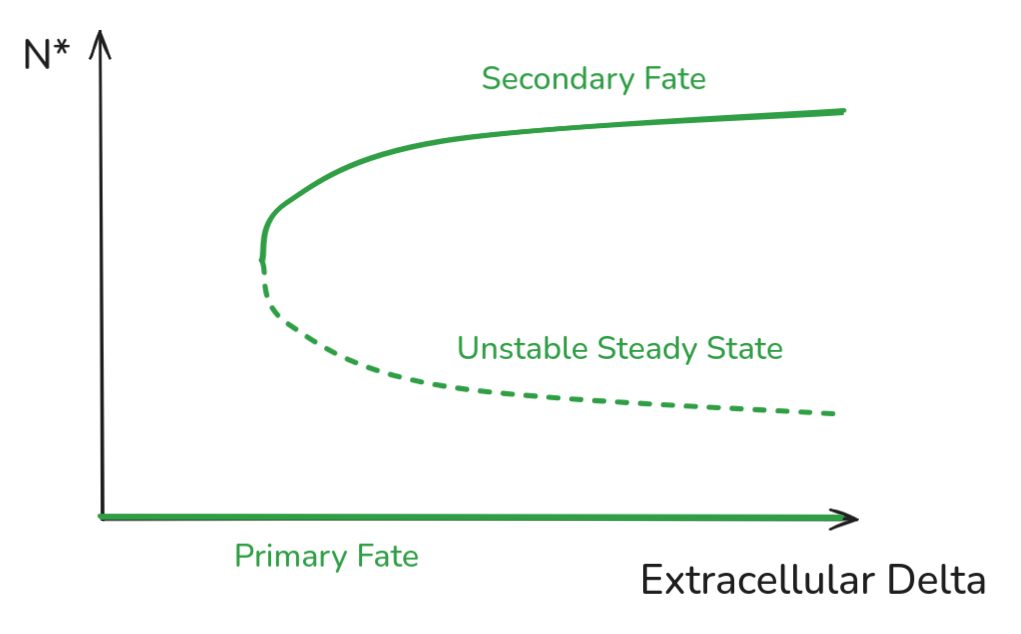
\includegraphics[width=\textwidth]{img/bifurcation-diagram.png}
  \caption{Approximate bifurcation diagram of the equilibrium Notch concentration of a single cell under the influence of fixed extracellular Delta from a neighbour.}
\end{figure}

\section{Results}

\subsection{Two-Cell Domain}

\begin{figure}
  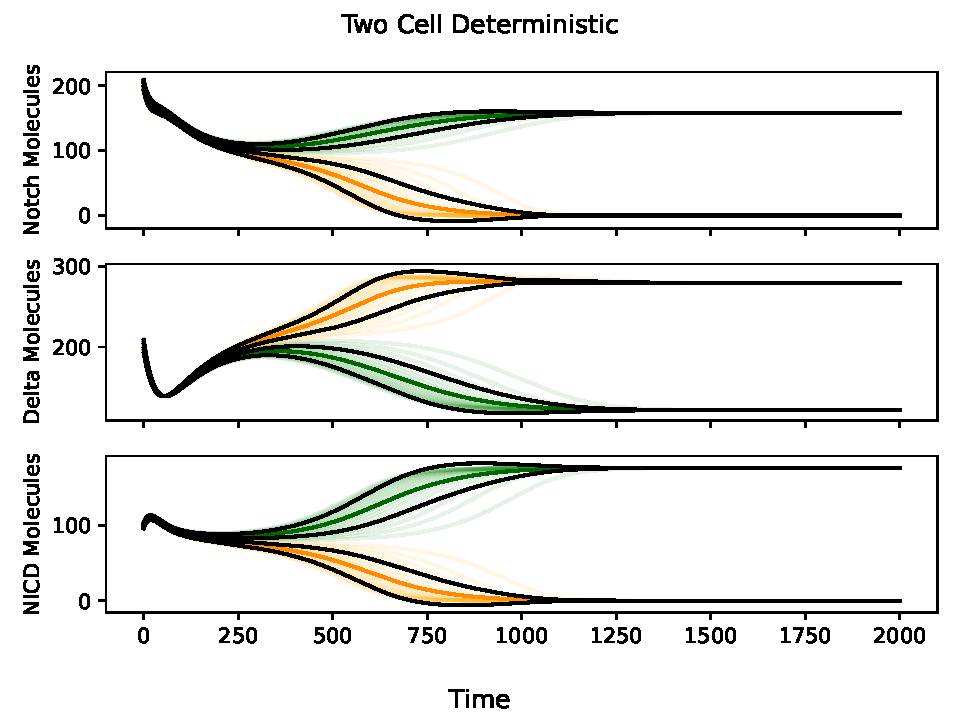
\includegraphics[width=\textwidth]{img/two_cell_deterministic.pdf}
  \caption{Results of the two-cell deterministic ODE model.}
\end{figure}

\begin{figure}
  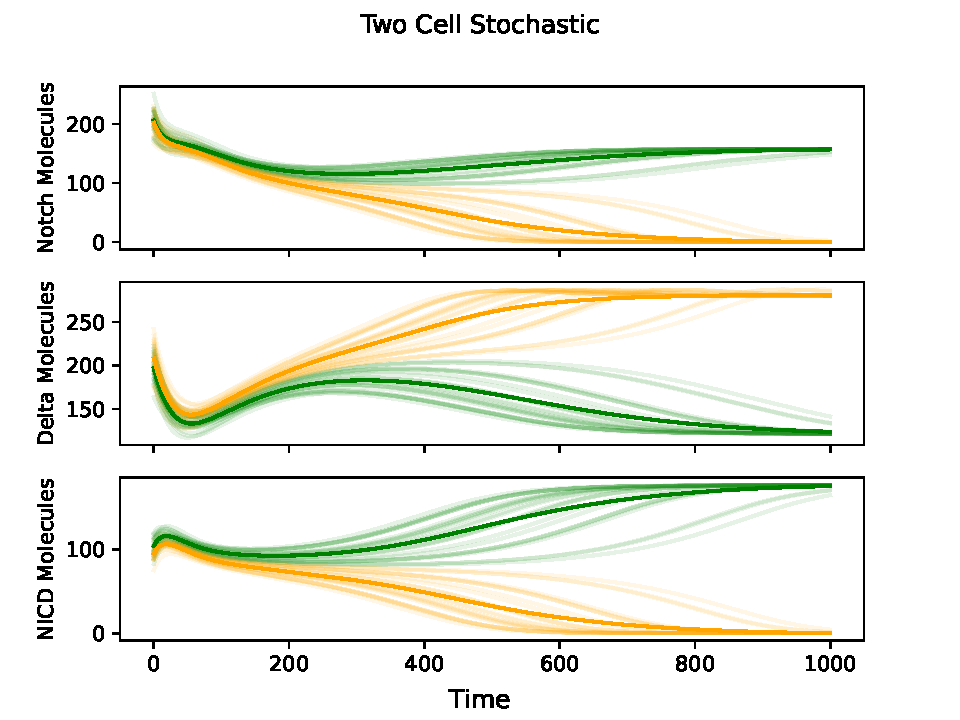
\includegraphics[width=\textwidth]{img/two_cell_stochastic.pdf}
  \caption{Results of the two-cell stochastic ODE model.}
\end{figure}

\begin{figure}
  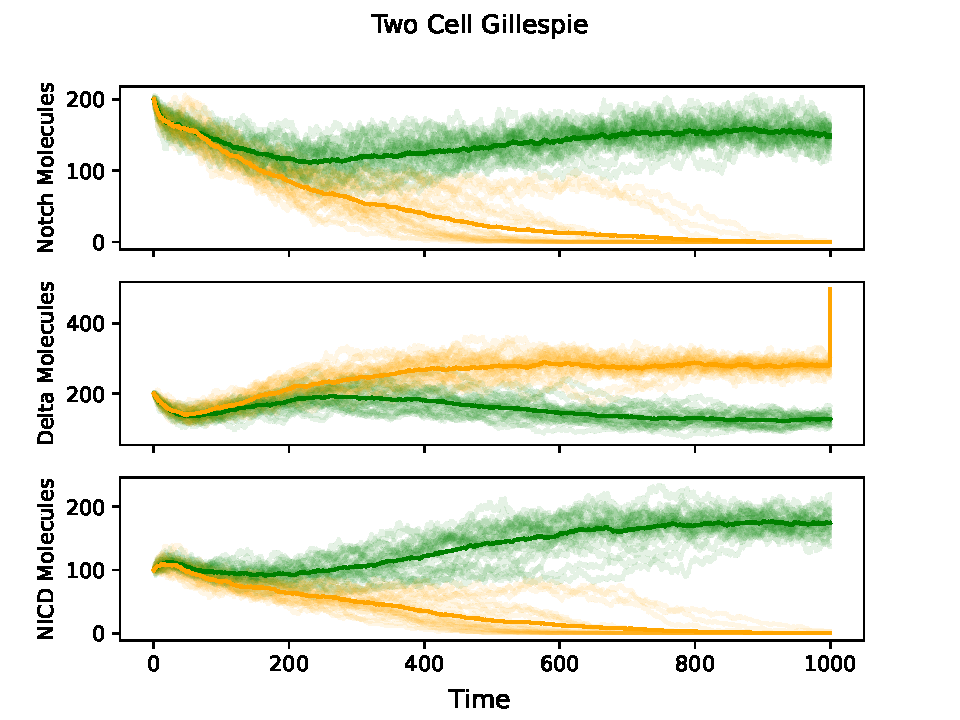
\includegraphics[width=\textwidth]{img/two_cell_gillespie.pdf}
  \caption{Results of the two-cell Gillespie model.}
\end{figure}

\begin{figure}
  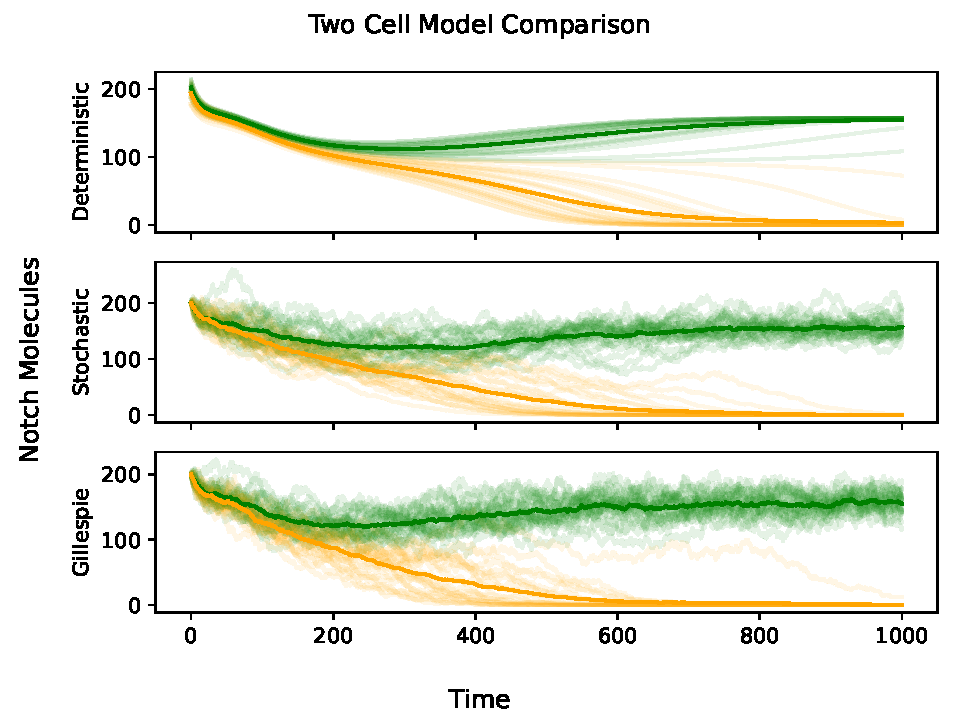
\includegraphics[width=\textwidth]{img/two_cell_comparison.pdf}
  \caption{Comparison of Notch concentrations in deterministic ODE, stochastic ODE, and Gillespie models. All models follow roughly the same trajectory and have similar differentiation times, although the Gillespie model appears to converge slightly faster.}
\end{figure}

\subsection{Linear Domain}

\begin{figure}
  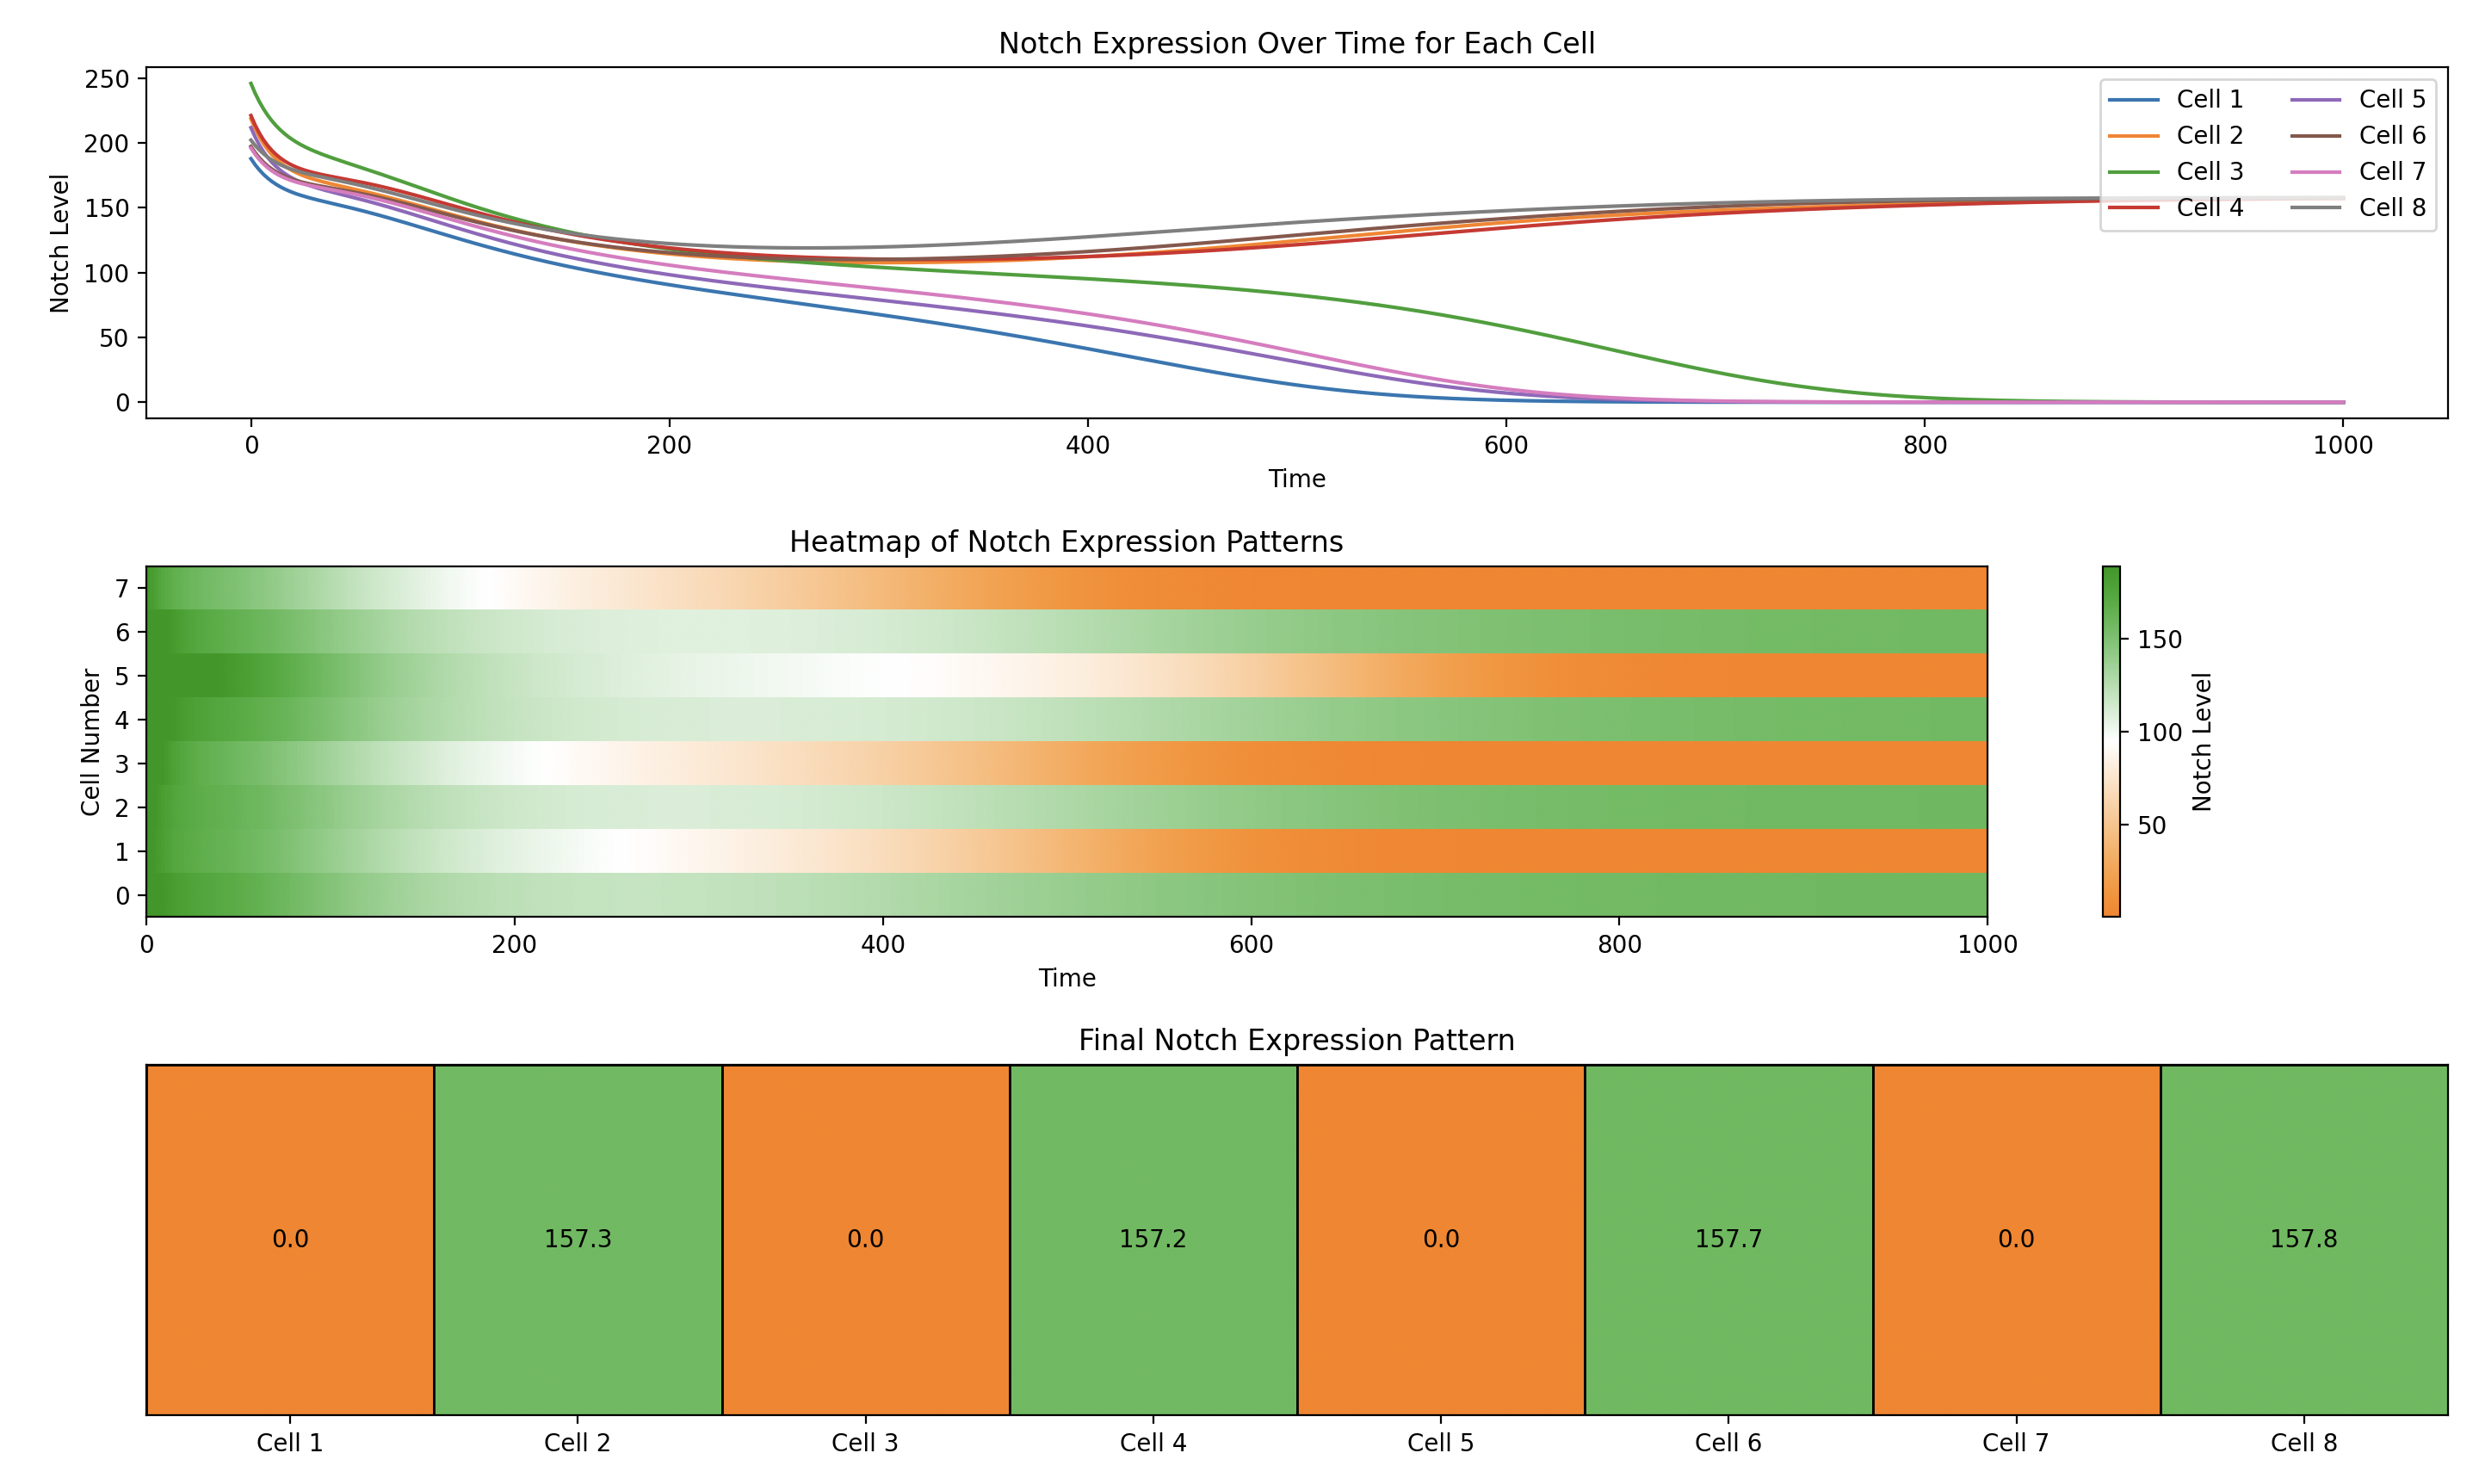
\includegraphics[width=\textwidth]{img/ODEModel_TwoCell_Heatmap.png}
  \caption{Results of the linear domain deterministic ODE model. Heatmap shows Notch levels in each of 8 cells over 1000 time steps.}
\end{figure}

\begin{figure}
  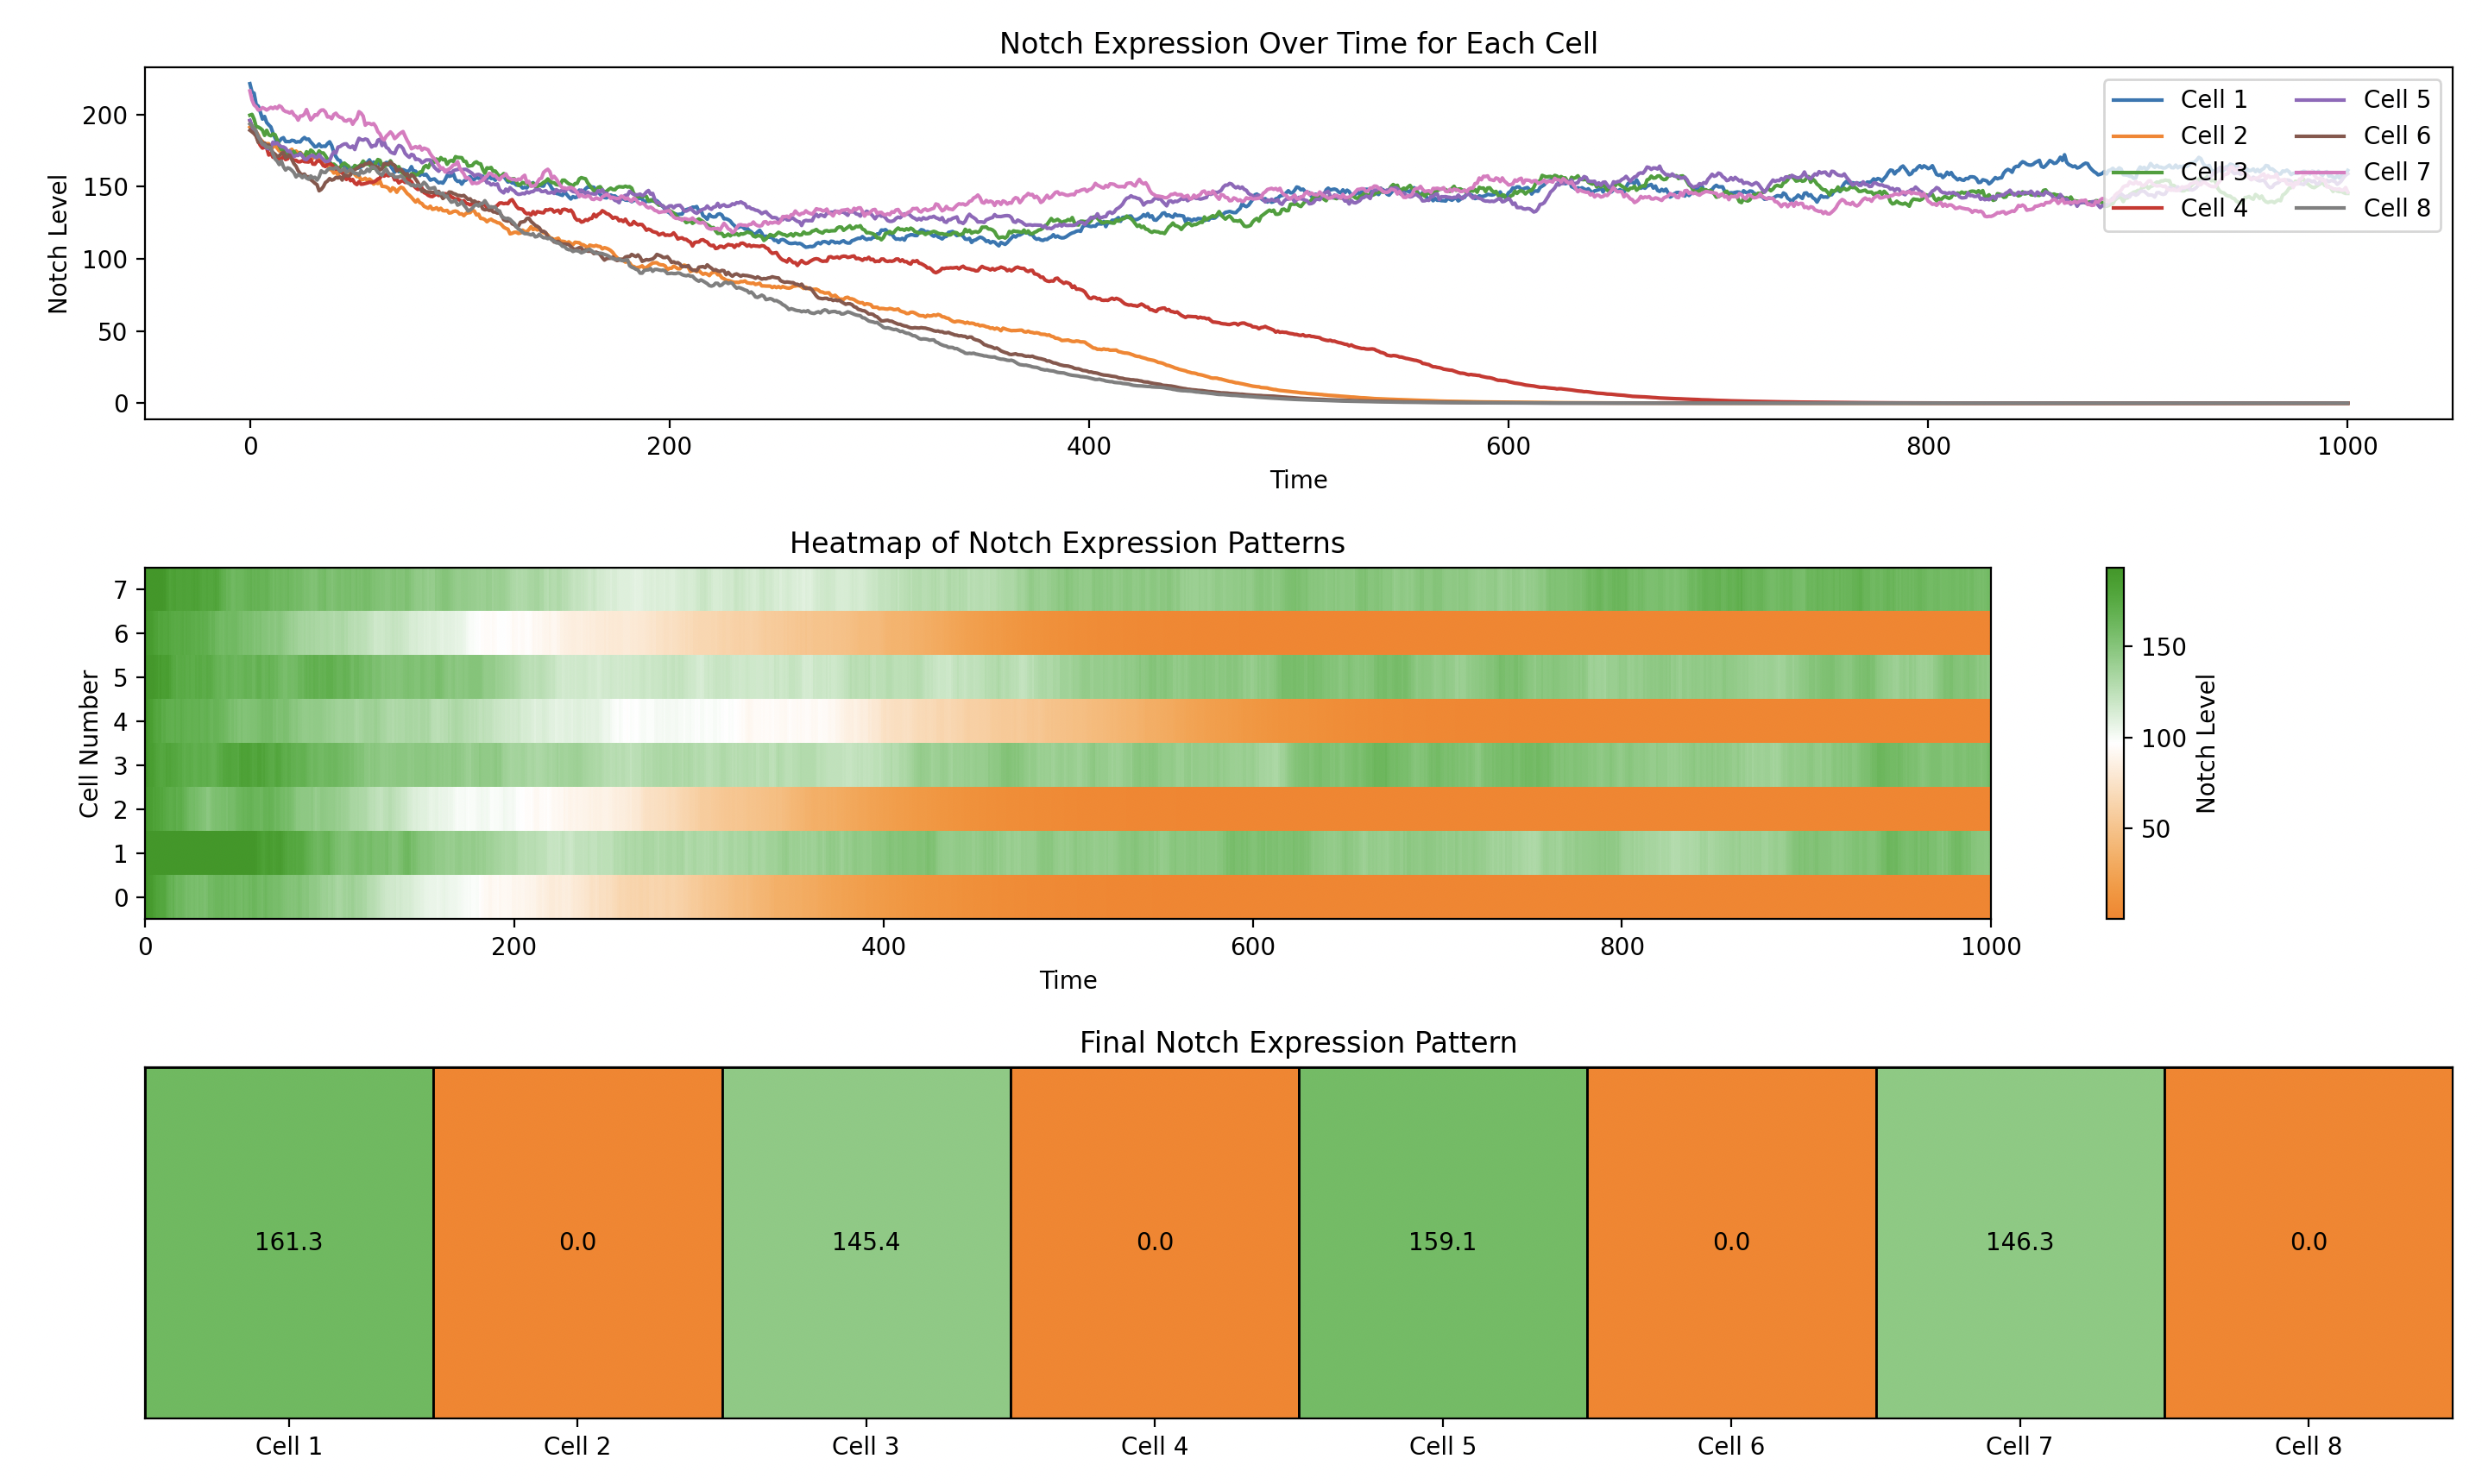
\includegraphics[width=\textwidth]{img/SDE_CellLine_HeatMap.png}
  \caption{Results of the linear domain SDE model. Heatmap shows Notch levels in each of 8 cells over 1000 time steps.}
\end{figure}

\subsection{Hexagonal Domain}

\begin{figure}
  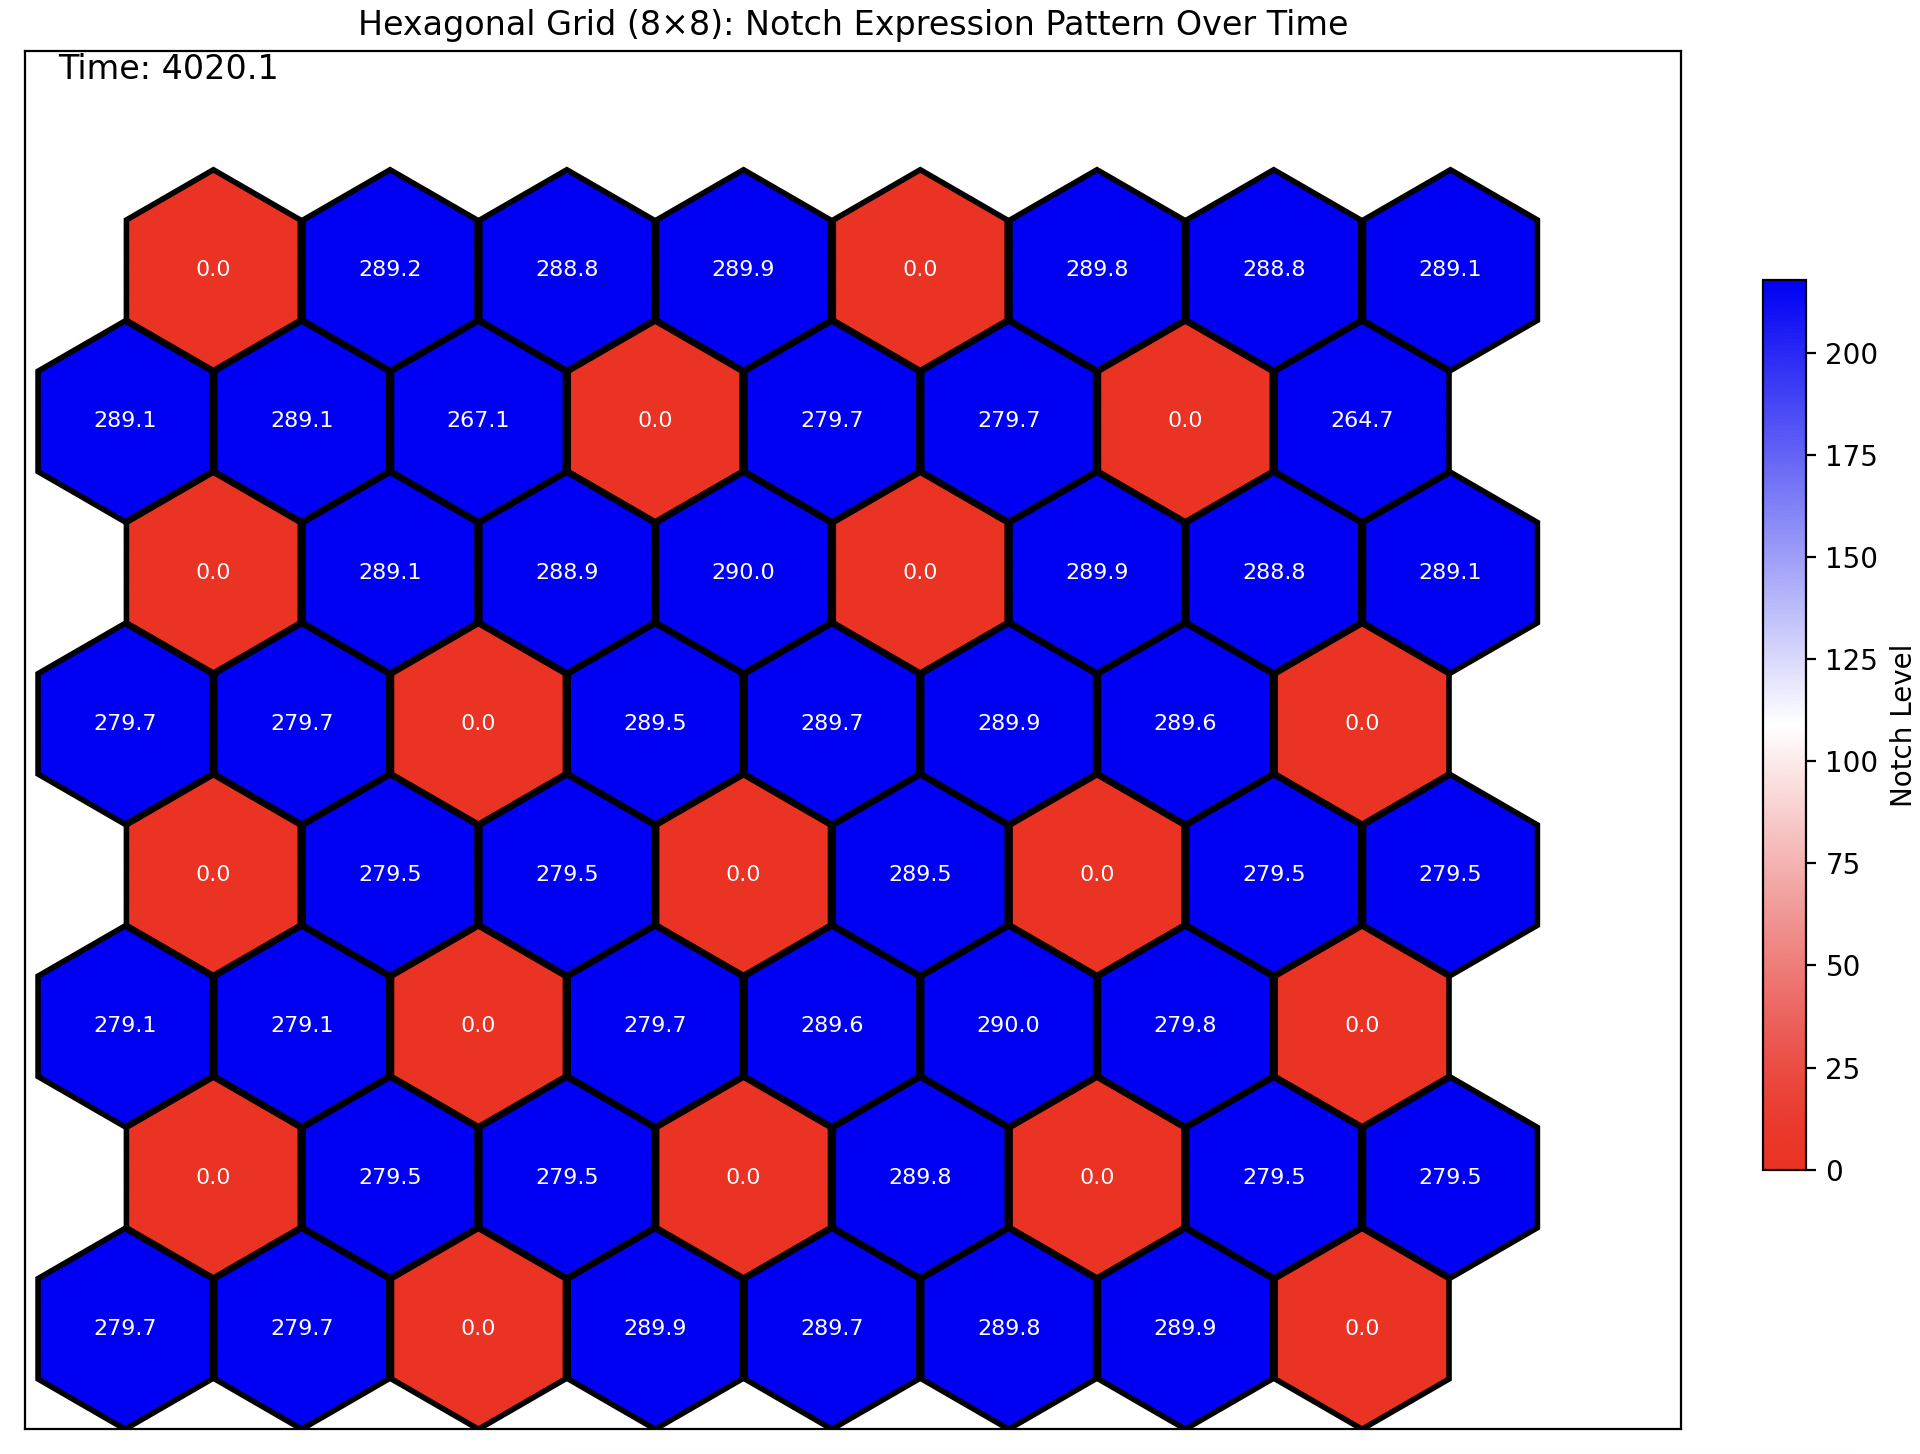
\includegraphics[width=\textwidth]{img/ODE_HexGrid.png}
  \caption{Results of the 8x8 hexagonal domain ODE model showing final Notch values per cell.}
\end{figure}

\section{Discussion}

\end{flushleft}

\nocite{*}
\printbibliography

\end{document}







